% Options for packages loaded elsewhere
\PassOptionsToPackage{unicode}{hyperref}
\PassOptionsToPackage{hyphens}{url}
%
\documentclass[
  french,
]{book}
\usepackage{lmodern}
\usepackage{amssymb,amsmath}
\usepackage{ifxetex,ifluatex}
\ifnum 0\ifxetex 1\fi\ifluatex 1\fi=0 % if pdftex
  \usepackage[T1]{fontenc}
  \usepackage[utf8]{inputenc}
  \usepackage{textcomp} % provide euro and other symbols
\else % if luatex or xetex
  \usepackage{unicode-math}
  \defaultfontfeatures{Scale=MatchLowercase}
  \defaultfontfeatures[\rmfamily]{Ligatures=TeX,Scale=1}
\fi
% Use upquote if available, for straight quotes in verbatim environments
\IfFileExists{upquote.sty}{\usepackage{upquote}}{}
\IfFileExists{microtype.sty}{% use microtype if available
  \usepackage[]{microtype}
  \UseMicrotypeSet[protrusion]{basicmath} % disable protrusion for tt fonts
}{}
\makeatletter
\@ifundefined{KOMAClassName}{% if non-KOMA class
  \IfFileExists{parskip.sty}{%
    \usepackage{parskip}
  }{% else
    \setlength{\parindent}{0pt}
    \setlength{\parskip}{6pt plus 2pt minus 1pt}}
}{% if KOMA class
  \KOMAoptions{parskip=half}}
\makeatother
\usepackage{xcolor}
\IfFileExists{xurl.sty}{\usepackage{xurl}}{} % add URL line breaks if available
\IfFileExists{bookmark.sty}{\usepackage{bookmark}}{\usepackage{hyperref}}
\hypersetup{
  pdftitle={Aide-mémoire : Analyses de données \& Cartographie sur R},
  pdfauthor={Alexis Mérot},
  pdflang={fr-FR},
  hidelinks,
  pdfcreator={LaTeX via pandoc}}
\urlstyle{same} % disable monospaced font for URLs
\usepackage{color}
\usepackage{fancyvrb}
\newcommand{\VerbBar}{|}
\newcommand{\VERB}{\Verb[commandchars=\\\{\}]}
\DefineVerbatimEnvironment{Highlighting}{Verbatim}{commandchars=\\\{\}}
% Add ',fontsize=\small' for more characters per line
\usepackage{framed}
\definecolor{shadecolor}{RGB}{248,248,248}
\newenvironment{Shaded}{\begin{snugshade}}{\end{snugshade}}
\newcommand{\AlertTok}[1]{\textcolor[rgb]{0.94,0.16,0.16}{#1}}
\newcommand{\AnnotationTok}[1]{\textcolor[rgb]{0.56,0.35,0.01}{\textbf{\textit{#1}}}}
\newcommand{\AttributeTok}[1]{\textcolor[rgb]{0.77,0.63,0.00}{#1}}
\newcommand{\BaseNTok}[1]{\textcolor[rgb]{0.00,0.00,0.81}{#1}}
\newcommand{\BuiltInTok}[1]{#1}
\newcommand{\CharTok}[1]{\textcolor[rgb]{0.31,0.60,0.02}{#1}}
\newcommand{\CommentTok}[1]{\textcolor[rgb]{0.56,0.35,0.01}{\textit{#1}}}
\newcommand{\CommentVarTok}[1]{\textcolor[rgb]{0.56,0.35,0.01}{\textbf{\textit{#1}}}}
\newcommand{\ConstantTok}[1]{\textcolor[rgb]{0.00,0.00,0.00}{#1}}
\newcommand{\ControlFlowTok}[1]{\textcolor[rgb]{0.13,0.29,0.53}{\textbf{#1}}}
\newcommand{\DataTypeTok}[1]{\textcolor[rgb]{0.13,0.29,0.53}{#1}}
\newcommand{\DecValTok}[1]{\textcolor[rgb]{0.00,0.00,0.81}{#1}}
\newcommand{\DocumentationTok}[1]{\textcolor[rgb]{0.56,0.35,0.01}{\textbf{\textit{#1}}}}
\newcommand{\ErrorTok}[1]{\textcolor[rgb]{0.64,0.00,0.00}{\textbf{#1}}}
\newcommand{\ExtensionTok}[1]{#1}
\newcommand{\FloatTok}[1]{\textcolor[rgb]{0.00,0.00,0.81}{#1}}
\newcommand{\FunctionTok}[1]{\textcolor[rgb]{0.00,0.00,0.00}{#1}}
\newcommand{\ImportTok}[1]{#1}
\newcommand{\InformationTok}[1]{\textcolor[rgb]{0.56,0.35,0.01}{\textbf{\textit{#1}}}}
\newcommand{\KeywordTok}[1]{\textcolor[rgb]{0.13,0.29,0.53}{\textbf{#1}}}
\newcommand{\NormalTok}[1]{#1}
\newcommand{\OperatorTok}[1]{\textcolor[rgb]{0.81,0.36,0.00}{\textbf{#1}}}
\newcommand{\OtherTok}[1]{\textcolor[rgb]{0.56,0.35,0.01}{#1}}
\newcommand{\PreprocessorTok}[1]{\textcolor[rgb]{0.56,0.35,0.01}{\textit{#1}}}
\newcommand{\RegionMarkerTok}[1]{#1}
\newcommand{\SpecialCharTok}[1]{\textcolor[rgb]{0.00,0.00,0.00}{#1}}
\newcommand{\SpecialStringTok}[1]{\textcolor[rgb]{0.31,0.60,0.02}{#1}}
\newcommand{\StringTok}[1]{\textcolor[rgb]{0.31,0.60,0.02}{#1}}
\newcommand{\VariableTok}[1]{\textcolor[rgb]{0.00,0.00,0.00}{#1}}
\newcommand{\VerbatimStringTok}[1]{\textcolor[rgb]{0.31,0.60,0.02}{#1}}
\newcommand{\WarningTok}[1]{\textcolor[rgb]{0.56,0.35,0.01}{\textbf{\textit{#1}}}}
\usepackage{longtable,booktabs}
% Correct order of tables after \paragraph or \subparagraph
\usepackage{etoolbox}
\makeatletter
\patchcmd\longtable{\par}{\if@noskipsec\mbox{}\fi\par}{}{}
\makeatother
% Allow footnotes in longtable head/foot
\IfFileExists{footnotehyper.sty}{\usepackage{footnotehyper}}{\usepackage{footnote}}
\makesavenoteenv{longtable}
\usepackage{graphicx}
\makeatletter
\def\maxwidth{\ifdim\Gin@nat@width>\linewidth\linewidth\else\Gin@nat@width\fi}
\def\maxheight{\ifdim\Gin@nat@height>\textheight\textheight\else\Gin@nat@height\fi}
\makeatother
% Scale images if necessary, so that they will not overflow the page
% margins by default, and it is still possible to overwrite the defaults
% using explicit options in \includegraphics[width, height, ...]{}
\setkeys{Gin}{width=\maxwidth,height=\maxheight,keepaspectratio}
% Set default figure placement to htbp
\makeatletter
\def\fps@figure{htbp}
\makeatother
\setlength{\emergencystretch}{3em} % prevent overfull lines
\providecommand{\tightlist}{%
  \setlength{\itemsep}{0pt}\setlength{\parskip}{0pt}}
\setcounter{secnumdepth}{5}
\usepackage{booktabs}
\usepackage{csquotes}
\usepackage[french]{babel} % Ajout du français
\usepackage{tcolorbox}

\newtcolorbox{blackbox}{
  colback=black!5!white,
  colframe=orange,
  coltext=black,
  boxsep=5pt,
  arc=4pt}

\newenvironment{infobox}[1]
  {
  \begin{itemize}
  \renewcommand{\labelitemi}{
    \raisebox{-.7\height}[0pt][0pt]{
      {\setkeys{Gin}{width=3em,keepaspectratio}
        \includegraphics{images/#1}}
    }
  }
  \setlength{\fboxsep}{1em}
  \begin{blackbox}
  \item
  }
  {
  \end{blackbox}
  \end{itemize}
  }
\ifxetex
  % Load polyglossia as late as possible: uses bidi with RTL langages (e.g. Hebrew, Arabic)
  \usepackage{polyglossia}
  \setmainlanguage[]{french}
\else
  \usepackage[shorthands=off,main=french]{babel}
\fi
\ifluatex
  \usepackage{selnolig}  % disable illegal ligatures
\fi
\usepackage[]{natbib}
\bibliographystyle{apalike}

\title{Aide-mémoire : Analyses de données \& Cartographie sur R}
\author{Alexis Mérot}
\date{Modifié le : 2020-08-06}

\begin{document}
\maketitle

{
\setcounter{tocdepth}{1}
\tableofcontents
}
\hypertarget{introduction}{%
\chapter*{Introduction}\label{introduction}}
\addcontentsline{toc}{chapter}{Introduction}

\begin{infobox}{caution}

Cet aide-mémoire n'est pour l'instant qu'un brouillon. Il est donc loin d'être complet et l'écriture est pour l'instant très succincte.

\end{infobox}

Ce projet est un ensemble de notes écrites en R Markdown \citep{R-rmarkdown} et via
le package \texttt{bookdown} (\url{https://github.com/rstudio/bookdown}). Ces notes
s'accumuleront au fur et à mesure de mon apprentissage des différents outils et
concepts dont j'ai besoin pour les analyses de données et la programmation. Cela
me permet de les comprendre, les mémoriser, ainsi que de les partager.

L'aide-mémoire s'insérera peut-être dans un autre plus gros projet : la création
d'un blog répertoriant tous mes projets et mon CV. Il commencera certainement
lorsque je pourrai démarrer la lecture de la documentation de l'excellent
package \texttt{blogdown} (\url{https://bookdown.org/yihui/blogdown/}).

Cet aide-mémoire intégrera les notions théoriques indispensables en statistique
et en cartographie, ainsi que les outils proposés par R (et si besoin d'autres
langages) pour la mise en pratique à travers d'exemples. Étant principalement
intéressé par la Biologie de la conservation et globalement l'Écologie, les
exemples se focaliseront pour la plupart sur des données en lien à ces domaines.

Toutes les sources qui m'ont été utiles pour acquérir ces connaissances seront
accessibles dans les références bibliographiques ou dans les ressources Internet
à la fin des chapitres.

Il n'y a pour l'instant qu'une version en ligne, mais une version PDF sera aussi disponible en téléchargement lorsque l'aide-mémoire sera plus mature.

\hypertarget{rmarkdown}{%
\chapter{R Markdown, Bookdown \& Blogdown}\label{rmarkdown}}

\begin{infobox}{caution}

\textbf{Work In Progress}

\end{infobox}

\hypertarget{pourquoi-rmarkdown}{%
\section{Pourquoi R Markdown ?}\label{pourquoi-rmarkdown}}

R Markdown désigne un format de fichier (à l'extension \textbf{.Rmd}) et plus
globalement le framework utilisé pour créer plus facilement des documents
(généralement scientifiques) automatisés. Ces documents peuvent ainsi être
totalement reproductibles et plusieurs formats de rendu final (statiques ou
dynamiques) sont supportés.

Le fichier est écrit via le langage Markdown et des sections de code R peuvent y
être insérées facilement (ainsi que du code écrit via d'autres langages tels
que Python ou SQL). Cela offre une syntaxe facile à lire et à écrire tout en
permettant de générer un document structuré et élégant.

Pour que cela fonctionne, R Markdown est lié à deux packages : \texttt{knitr} et le
convertisseur universel de document \texttt{pandoc} (Fig. \ref{fig:rmarkdownflow}).\\
Le package \texttt{knitr} permet la création, à partir du fichier \textbf{.Rmd}, d'un fichier
au format \textbf{md} contenant le code et sa sortie. Ce fichier est alors converti
dans le format de rendu final voulu via \texttt{pandoc} (\textbf{.html}, \textbf{.pdf}, etc).



\begin{figure}

{\centering 
\includegraphics[width=0.6\linewidth]{images/rmarkdownflow} 

}

\caption{\emph{Source : \url{https://rmarkdown.rstudio.com/lesson-2.html}}}\label{fig:rmarkdownflow}
\end{figure}

Toutes mes notes seront donc écrites via R Markdown, et cette section intégrera
toutes les astuces intéressantes que je rencontre au fur et à mesure des
besoins.

Pour ne pas paraphraser tout l'excellent guide de \citet{rmarkdown2018}, je vous invite à
lire leur excellent guide gratuit : \url{https://bookdown.org/yihui/rmarkdown/},
ainsi que le livre en cours d'écriture
\href{https://bookdown.org/yihui/rmarkdown-cookbook/}{R Markdown Cookbook}.

\begin{center}\rule{0.5\linewidth}{0.5pt}\end{center}

\hypertarget{ref-rmd}{%
\section*{Liste de ressources Internet utiles}\label{ref-rmd}}
\addcontentsline{toc}{section}{Liste de ressources Internet utiles}

\begin{itemize}
\tightlist
\item
  R Markdown :

  \begin{itemize}
  \tightlist
  \item
    \href{https://rmarkdown.rstudio.com/lesson-1.html}{Vue d'ensemble} de R Markdown
  \item
    \href{https://ysc-rmarkdown.netlify.app/}{Cours} sur la communication avec R Markdown
  \item
    \href{https://emilyriederer.netlify.app/post/rmarkdown-driven-development/}{Comment utiliser R Markdown}
    comme base pour le développement de packages bien organisés
  \item
    Quelques \href{https://www.dataquest.io/blog/r-markdown-tips-tricks-and-shortcuts/}{trucs et astuces}
    sur R Markdown
  \item
    \href{https://holtzy.github.io/Pimp-my-rmd/}{Comment donner du \emph{peps}}
    à mon document RMD
  \item
    \href{https://www.dataquest.io/blog/r-markdown-guide-cheatsheet/}{Un autre guide}
    de R Markdown
  \item
    \href{https://bookdown.org/yihui/rmarkdown/}{Guide complet} de R Markdown
  \item
    \href{https://bookdown.org/yihui/rmarkdown-cookbook/}{Nouveau guide}
    de R Markdown (\textbf{\emph{en cours d'écriture}})
  \item
    \href{https://danawanzer.com/using-r-for-immediate-reporting-in-evaluation/}{Création d'un template}
    R Markdown
  \end{itemize}
\item
  Bookdown :

  \begin{itemize}
  \tightlist
  \item
    \href{https://bookdown.org/home/about/}{Site officiel} de \texttt{bookdown}
  \item
    \href{https://bookdown.org/yihui/bookdown/}{Guide complet} de \texttt{bookdown}
  \item
    Extension à \texttt{bookdown} : \href{https://bookdown.org/baydap/bookdownplus/}{\texttt{bookdownplus}}
  \item
    \href{https://statistique-et-logiciel-r.com/creer-un-livre-document-avec-bookdown/}{Guide en français}
    de \texttt{bookdown}
  \item
    \href{https://thinkr.fr/rediger-avec-bookdown-pourquoi-comment/}{Introduction en français}
    à \texttt{bookdown}
  \end{itemize}
\item
  Blogdown :

  \begin{itemize}
  \tightlist
  \item
    \href{https://bookdown.org/yihui/blogdown/}{Guide complet} sur \texttt{blogdown}
  \end{itemize}
\item
  Court \href{https://slides.yihui.org/2017-rmarkdown-UNL-Yihui-Xie.html\#1}{tutoriel}
  d'introduction sur R Markdown, \texttt{bookdown} et \texttt{blogdown}
\item
  Guide pour le package \href{https://yihui.org/knitr/}{\texttt{knitr}}
\item
  \href{https://yihui.org/knitr/options/}{Options} valables pour les \emph{chunks} de code
  et le package \texttt{knitr}
\end{itemize}

\begin{center}\rule{0.5\linewidth}{0.5pt}\end{center}

\hypertarget{data-analysis}{%
\chapter{Extraction/importation, nettoyage \& manipulation des données}\label{data-analysis}}

\begin{infobox}{caution}

\textbf{Work In Progress}

\end{infobox}

\hypertarget{extraction-de-donnuxe9es-provenant-dun-pdf}{%
\section{Extraction de données provenant d'un PDF}\label{extraction-de-donnuxe9es-provenant-dun-pdf}}

\hypertarget{ruxe9cupuxe9ration-de-donnuxe9es-provenant-du-web-le-web-scraping}{%
\section{\texorpdfstring{Récupération de données provenant du web : le \emph{web scraping}}{Récupération de données provenant du web : le web scraping}}\label{ruxe9cupuxe9ration-de-donnuxe9es-provenant-du-web-le-web-scraping}}

\hypertarget{ref-data-analysis}{%
\section*{Liste de ressources Internet utiles}\label{ref-data-analysis}}
\addcontentsline{toc}{section}{Liste de ressources Internet utiles}

\hypertarget{statistique}{%
\chapter{Statistique}\label{statistique}}

\begin{infobox}{caution}

\textbf{Work In Progress}

\end{infobox}

\hypertarget{quelques-notions-cluxe9s}{%
\section{Quelques notions clés}\label{quelques-notions-cluxe9s}}

Concepts à comprendre :

\begin{itemize}
\tightlist
\item
  Théorie des probabilités
\item
  Variable aléatoire réelle
\item
  Fonction de répartition (ou fonction de distribution cumulative) d'une
  variable aléatoire
\item
  Fonction de densité ou densité de probabilité
\end{itemize}

\hypertarget{frequentiste}{%
\section{Statistique fréquentiste}\label{frequentiste}}

\begin{center}\rule{0.5\linewidth}{0.5pt}\end{center}

\hypertarget{ref-stat-freq}{%
\section*{Liste de ressources Internet utiles}\label{ref-stat-freq}}
\addcontentsline{toc}{section}{Liste de ressources Internet utiles}

\begin{center}\rule{0.5\linewidth}{0.5pt}\end{center}

\hypertarget{bayesienne}{%
\section{Statistique bayésienne}\label{bayesienne}}

\begin{center}\rule{0.5\linewidth}{0.5pt}\end{center}

\hypertarget{ref-stat-bayes}{%
\section*{Liste de ressources Internet utiles}\label{ref-stat-bayes}}
\addcontentsline{toc}{section}{Liste de ressources Internet utiles}

\begin{center}\rule{0.5\linewidth}{0.5pt}\end{center}

\hypertarget{dataviz}{%
\chapter{\texorpdfstring{Visualisation des données : la \emph{Dataviz}}{Visualisation des données : la Dataviz}}\label{dataviz}}

\begin{infobox}{caution}

\textbf{Work In Progress}

\end{infobox}

\hypertarget{SIG}{%
\chapter{Les Systèmes d'Information Géographiques}\label{SIG}}

\begin{infobox}{caution}

\textbf{Work In Progress}

\end{infobox}

\hypertarget{quest-ce-quun-sig}{%
\section{Qu'est-ce qu'un SIG ?}\label{quest-ce-quun-sig}}

Un Système d'Information Géographique est, comme tout Système d'Information
\footnote{Cf. le cours sur
  \href{https://openclassrooms.com/fr/courses/2100086-decouvrez-le-monde-des-systemes-dinformation}{Openclassroom}.}, un ensemble organisé de ressources ayant pour fonction de collecter,
stocker, traiter et diffuser des informations \footnote{Cf. la page Wikipédia sur le
  \href{https://fr.wikipedia.org/wiki/Syst\%C3\%A8me_d\%27information_g\%C3\%A9ographique}{Système d'Information Géographique}.}. Ici, ces informations
(généralement informatisées) sont des données géospatiales stockées sous forme
de couches d'informations superposées et reliées les unes aux autres par un
référentiel cartographique \footnote{Fond de carte représentant un territoire géographique sur lequel
  peuvent s'appuyer de nouvelles données cartographiques.}. Les SIG sont devenus des outils
essentiels dans de nombreux domaines tels que l'écologie, la médecine ou la
sociologie.

Pour aider les utilisateurs au traitement des données géospatiales, il existe de
performants et très utilisés logiciels gratuits ou payants tels que
\href{https://www.qgis.org/fr/site/}{QGis} ou
\href{https://www.arcgis.com/index.html}{ArcGIS}. Ces logiciels offrent une approche
graphique à la lecture, l'écriture, la manipulation et la visualisation des
données. Ceci peut néanmoins limiter la reproductibilité et l'automatisation des
projets. Pour remédier à cela, de nombreux langages de programmation peuvent
être utilisés pour écrire et partager des scripts. Parmi les plus utilisés, il y
a \href{https://www.python.org/}{Python} (qui est notamment utilisé pour la
conception de plugins dans les logiciels de SIG) et
\href{https://www.r-project.org/about.html}{R} (dont les scripts sont maintenant
exécutables dans QGis). En plus de cela, l'approche en lignes de commande permet
de se libérer de certaines contraintes imposées par ces logiciels ainsi que
d'avoir plus de contrôle sur ce que l'ont fait (même si ces logiciels sont de
plus en plus performants).

\hypertarget{r-en-tant-que-sig}{%
\section{R en tant que SIG}\label{r-en-tant-que-sig}}

Afin d'avoir un bon aperçu et une bonne base sur l'utilisation de R en tant que
SIG, je vous invite à lire le livre \emph{Geocomputation with R} de \citet{geocomputation}.
Ce livre est mis à jour régulièrement et consultable gratuitement à cette
adresse : \url{https://geocompr.robinlovelace.net/}. Si vous préférez le format
papier et/ou voulez soutenir les auteurs, il est bien sûr disponible à l'achat.

Ayant commencé à apprendre les analyses statistiques avec R, c'est naturellement
que je me suis tourné vers ce langage pour la cartographie et l'analyse des
données géospatiales. En effet, la communauté de R a créé de performants et
magnifiques packages de cartographie et de géocalcul libres, gratuits et bien
documentés. Je m'intéresserai donc de plus près à ce qu'offre par exemple Python
lorsque j'aurai maîtrisé suffisamment R. Un autre langage élégant et très récent
qui est à regarder de très près est \href{https://julialang.org/}{Julia}, qui offrira
certainement des packages rapides et performants au fur et à mesure de sa
maturité. Par ailleurs, même si des programmes manqueraient à R ou si d'autres
langages possèdent des programmes plus adaptés pour certaines tâches, des
packages R offrent la possibilité d'en faciliter l'accès. Par exemple, les
packages tels que \href{https://github.com/RcppCore/Rcpp}{\texttt{Rcpp}} et
\href{https://rstudio.github.io/reticulate/}{\texttt{Reticulate}} permettent l'utilisation
de programmes écrits respectivement en C++ et Python.

D'autres caractéristiques intéressantes de R sont sa flexibilité et sa constante
évolution. Par exemple, il offre maintenant la possibilité de faire facilement
des applications web et des cartes interactives notamment via les packages
\href{https://shiny.rstudio.com/}{\texttt{Shiny}} et
\href{https://rstudio.github.io/leaflet/}{\texttt{Leaflet}}. Il offre par la même occasion
divers outils d'analyses avancées, de modélisation et de visualisation qui sont
mis à jour et améliorés régulièrement.

Pour plus d'informations concernant les atouts de R en tant que SIG ainsi qu'un
bref aperçu de l'utilité des autres langages tels que Python, Java et C++, je
vous invite à lire le chapitre \href{https://geocompr.robinlovelace.net/intro.html\#why-use-r-for-geocomputation}{Why use R for
geocomputation}
du livre de \citet{geocomputation}.

\hypertarget{la-repruxe9sentation-des-donnuxe9es-les-vecteurs-et-les-rasters}{%
\section{\texorpdfstring{La représentation des données : les \emph{vecteurs} et les \emph{rasters}}{La représentation des données : les vecteurs et les rasters}}\label{la-repruxe9sentation-des-donnuxe9es-les-vecteurs-et-les-rasters}}

Pour représenter numériquement les données spatiales, deux modèles de base sont
utilisés : les \emph{vecteurs} (mode vectoriel) et les \emph{rasters} (mode matriciel).
L'une des principales différences entre ces deux modèles est qu'un vecteur est
un \emph{objet} (ou entité) tandis que le raster est une \emph{image}. Ainsi, les vecteurs
sont constitués de points, de lignes et de polygones créés à partir d'équations
mathématiques, tandis que les rasters sont des grilles constituées de cellules
de même taille (les pixels). C'est cette différence qui fait que les vecteurs ne
perdent pas en netteté lorsque l'on zoome dessus, tandis que les images
deviennent floues (elles « pixelisent »). Par ailleurs, la différence dans la
manière de stocker ces deux modèles fait que les fichiers liés aux vecteurs ont
une taille bien inférieure que ceux liés aux raster.\\
Sous R, les vecteurs et les rasters sont travaillés respectivement avec les packages \texttt{sf} et \texttt{raster}.

\hypertarget{les-vecteurs}{%
\subsection{Les vecteurs}\label{les-vecteurs}}

Un vecteur est une image vectorielle ou dessin mathématique constitué de deux
composantes : une \textbf{composante attributaire} permettant de l'identifier, et une
\textbf{composante graphique} décrivant sa géométrie. Il est localisé grâce à un
système de coordonnées spatiales (ou CRS pour \emph{Coordinate Reference System} en
anglais). Les vecteurs sont basiquement composés de nœuds ou sommets qui sont
des \textbf{points dans l'espace}. À partir de ces sommets, des \textbf{formules
mathématiques} sont appliquées pour créer des \textbf{formes géométriques}. S'il n'y
a qu'un sommet, le vecteur est simplement un point. S'il y a plusieurs sommets
et que les liaisons ne forment pas une forme géométrique fermée, alors cela
forme une ligne. Si la forme est fermée, le vecteur est un polygone. La
géométrie des points est généralement en deux dimensions (\(x =\) longitude, \(y =\)
latitude), mais peut être parfois en trois dimensions si une valeur \(z\)
additionnelle est ajoutée (notamment pour représenter la hauteur au-dessus du
niveau de la mer).\\
Les vecteurs permettent donc de représenter des \textbf{données discrètes} avec des
\textbf{formes bien définies dans l'espace}.

Pour stocker la géométrie de ces \textbf{entités géographiques},
l'OGC \footnote{L'OGC est un consortium international qui développe des standards ouverts
  (OpenGIS) dans les domaines de la géomatique et de l'information géographique.} (\href{https://www.ogc.org/}{\emph{Open Geospatial Consortium}}) a développé
un modèle standardisé pour les Bases de Données Spatiales (BDS). Ce modèle
s'appelle \textbf{Modèle d'Entité Simple} (SFA pour \href{https://www.ogc.org/standards/sfa}{\emph{Simple Feature
Access}} en anglais) et permet de définir des
fonctions pour accéder, faire des calculs et construire les données, dans le but
de représenter les objets dans la réalité. C'est un modèle de données très
largement supportés dans la plupart des logiciels SIG (dont QGIS) et a
l'avantage de rendre le travail totalement transférable d'un projet à un autre
grâce à une architecture commune.

Pour amener ce modèle dans R, le package \texttt{sf} a ainsi été créé pour succéder au
package \texttt{sp} sur le long terme \footnote{Cf. la \href{https://r-spatial.github.io/sf/articles/sf1.html}{vignette}
  du package \texttt{sf} parlant de ce sujet.}. Les différents \textbf{types de
géométrie} définis par la norme standardisée de l'OGC sont donc inclus dans ce
package (fig.~\ref{fig:sfclasses}). Ces types de géométrie permettent de créer les
entités, qui sont la \textbf{représentation d'un objet dans le monde réel} (comme un
bâtiment, un champ ou un arbre). Chaque entité peut alors faire parti par
exemple du type \texttt{POINT}, \texttt{POLYLIGNE} (\texttt{LINESTRING}) ou \texttt{POLYGONE}. En plus de
cela, il est possible de créer d'autres entités à partir de l'agrégation de ces
entités basiques (formant des \texttt{MULITPOINTS}, des \texttt{MULTIPOLYLIGNES} et des
\texttt{MULTIPOLYGONES}). Une seule entité contenant plusieurs types de géométrie
différents est alors de type « collection de géométrie » (\texttt{GEOMETRYCOLLECTION}).\\
Ces 7 types de géométrie précédemment cités font partis des types les plus
utilisés. Dans le package \texttt{sf}, ces types sont représentés sous la forme de
\emph{classes}.



\begin{figure}

{\centering 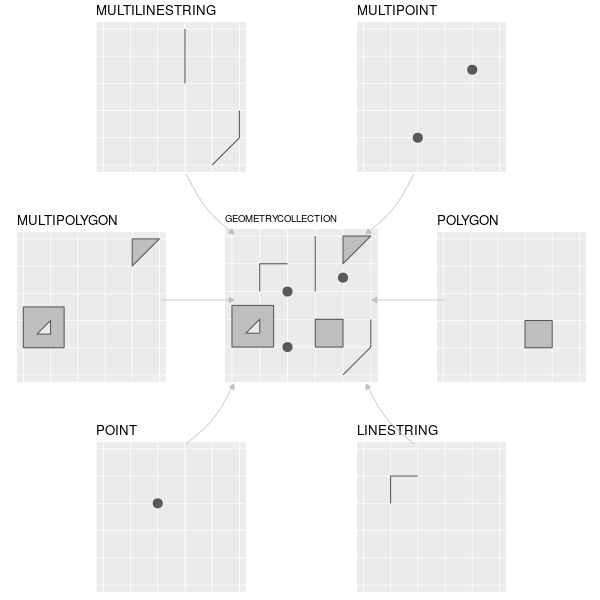
\includegraphics[width=0.6\linewidth]{images/sf-classes} 

}

\caption{Exemple des différents types de géométrie supportés par le package \texttt{sf} (source : \url{https://geocompr.robinlovelace.net/spatial-class.html\#intro-sf})}\label{fig:sfclasses}
\end{figure}

Le package \texttt{sf} est multitâche, il permet de : lire et écrire des fichiers de
données spatiales via la bibliothèque
\href{https://www.osgeo.org/projects/geos/}{GEOS} ; faire des opérations géométriques
via la bibliothèque \href{https://gdal.org/}{GDAL} ; mais aussi représenter et
transformer des systèmes de coordonnées géographiques projetés via la
bibliothèque \href{https://proj.org/}{PROJ}.

Pour commencer, nous allons prendre pour exemple le jeu de données \texttt{world} du
package \texttt{sf}. Ce jeu de données provenant de \href{https://www.naturalearthdata.com/}{Natural
Earth} est un objet \texttt{sf} contenant la carte
du monde ainsi que quelques données de banques mondiales (tableau
\ref{tab:dataworld}).



\begin{Shaded}
\begin{Highlighting}[]
\NormalTok{knitr}\OperatorTok{::}\KeywordTok{kable}\NormalTok{(}\KeywordTok{head}\NormalTok{(world), }\DataTypeTok{caption =} \StringTok{"Aperçu du jeu de données \texttt{world} inclus dans le package \texttt{spData}."}\NormalTok{) }\OperatorTok{\%\textgreater{}\%}
\StringTok{  }\NormalTok{kableExtra}\OperatorTok{::}\KeywordTok{kable\_styling}\NormalTok{(}
    \DataTypeTok{latex\_options =} \KeywordTok{c}\NormalTok{(}\StringTok{"striped"}\NormalTok{, }\StringTok{"hovered"}\NormalTok{, }\StringTok{"condensed"}\NormalTok{, }\StringTok{"responsive"}\NormalTok{)}
\NormalTok{  ) }\OperatorTok{\%\textgreater{}\%}
\StringTok{  }\NormalTok{kableExtra}\OperatorTok{::}\KeywordTok{scroll\_box}\NormalTok{(}\DataTypeTok{width =} \StringTok{"100\%"}\NormalTok{)}
\end{Highlighting}
\end{Shaded}

\label{tab:dataworld}Aperçu du jeu de données \texttt{world} inclus dans le package \texttt{spData}.

iso\_a2

name\_long

continent

region\_un

subregion

type

area\_km2

pop

lifeExp

gdpPercap

geom

FJ

Fiji

Oceania

Oceania

Melanesia

Sovereign country

19289.97

885806

69.96000

8222.254

MULTIPOLYGON (((180 -16.067\ldots{}

TZ

Tanzania

Africa

Africa

Eastern Africa

Sovereign country

932745.79

52234869

64.16300

2402.099

MULTIPOLYGON (((33.90371 -0\ldots{}

EH

Western Sahara

Africa

Africa

Northern Africa

Indeterminate

96270.60

NA

NA

NA

MULTIPOLYGON (((-8.66559 27\ldots{}

CA

Canada

North America

Americas

Northern America

Sovereign country

10036042.98

35535348

81.95305

43079.143

MULTIPOLYGON (((-122.84 49,\ldots{}

US

United States

North America

Americas

Northern America

Country

9510743.74

318622525

78.84146

51921.985

MULTIPOLYGON (((-122.84 49,\ldots{}

KZ

Kazakhstan

Asia

Asia

Central Asia

Sovereign country

2729810.51

17288285

71.62000

23587.338

MULTIPOLYGON (((87.35997 49\ldots{}

\hypertarget{les-rasters}{%
\subsection{Les rasters}\label{les-rasters}}

Un raster représente une image constituée de pixels (cellules) organisé(e)s sous
la forme d'une grille. C'est la représentation que l'on a l'habitude de voir
lorsque l'on parle d'une image numérique. Chaque pixel est unique et possède
certaines valeurs le caractérisant (comme sa couleur, ses coordonnées, son
altitude\ldots). Les données sont ainsi organisées en \textbf{matrice}, où chaque
\textbf{cellule} correspond à un pixel. Pour bien superposer le raster à la carte,
les matrices possèdent une en-tête incluant le \textbf{système de coordonnées
spatiales}, \textbf{l'origine} (généralement les coordonnées du coin inférieur droit
de la matrice), ainsi que l'\textbf{étendue de la matrice} (le nombre de colonnes, de
lignes et la résolution spatiale \footnote{Globalement, la résolution spatiale est la \textbf{taille réelle du
  plus petit élément} représenté dans un jeu de données. Pour le \emph{mode
  matriciel}, cela \textbf{correspond à la taille de la cellule de la grille}. Par
  exemple, si une cellule représente une surface réelle de 10 x 10 m, alors la
  résolution est de 10 m. La résolution spatiale permet donc de \textbf{définir le
  niveau de détail} du jeu de données. La netteté de l'image est ainsi dépendante
  de la résolution spatiale puisqu'il y aura plus de détails capturés avec des
  cellules de petite taille (résolution élevée ou fine) qu'avec des cellules de
  grande taille (résolution basse ou grossière).}).\\
De par leurs caractéristiques, les rasters permettent de définir des \textbf{données
discrètes} ainsi que des \textbf{données continues}.

\begin{center}\rule{0.5\linewidth}{0.5pt}\end{center}

\hypertarget{ref-sig}{%
\section*{Liste de ressources Internet utiles}\label{ref-sig}}
\addcontentsline{toc}{section}{Liste de ressources Internet utiles}

\begin{itemize}
\tightlist
\item
  \href{https://geocompr.robinlovelace.net/}{Guide} sur les analyses de données
  géographiques, leur visualisation et leur modélisation sur R
\item
  \href{https://statnmap.com/2018-07-14-introduction-to-mapping-with-sf-and-co/}{Introduction}
  à l'utilisation des packages de cartographie sur R
\item
  \href{https://www.infoworld.com/article/3505897/how-to-do-spatial-analysis-in-r-with-sf.amp.html}{Introduction}
  au package \texttt{sf}
\item
  \href{https://github.com/r-spatial/mapedit}{Édition} interactive de cartes avec
  \texttt{mapedit}
\item
  \href{https://mhallwor.github.io/_pages/welcome}{introduction} à l'utilisation de R
  comme un SIG
\item
  \href{http://eriqande.github.io/rep-res-web/lectures/making-maps-with-R.html}{Introduction}
  pour créer des cartes avec R
\item
  \href{https://thinkr.fr/sil-te-plait-dessine-moi-carte-r/}{Introduction}
  en français pour créer des cartes avec R
\item
  Introduction en français sur le package
  \href{https://colinfay.me/carte-r-rgeoapi-ggplot2/}{\texttt{rgeoapi}}
\item
  \href{https://rgeomatic.hypotheses.org/tag/sf}{Zoomer} sur une carte avec R
\item
  \href{https://rpubs.com/huanfaChen/ggplotShapefile}{Tracer des cartes avec \texttt{ggplot2}}
  via des fichiers \emph{shapefiles}
\item
  \href{https://www.r-spatial.org/r/2018/10/25/ggplot2-sf.html}{Tutoriel}
  pour dessiner des cartes avec R, \texttt{sf} et \texttt{ggplot2}
\item
  \href{https://r-spatial.github.io/mapview/}{Cartes interactives} avec \texttt{mapview}
\item
  \href{https://rstudio.github.io/leaflet/}{Cartes interactives} avec \texttt{leaflet}
\item
  Guide pour faire des
  \href{https://www.tylermw.com/a-step-by-step-guide-to-making-3d-maps-with-satellite-imagery-in-r/}{cartes en 3D}
  à partir d'une imagerie satellite
\item
  Utilisation du package \href{https://www.rayshader.com/}{\texttt{rayshader}} pour la
  création de cartes en 2D et 3D
\item
  Manipulation et visualisation de données
  \href{https://github.com/Jean-Romain/lidR}{LiDAR} pour la foresterie avec \texttt{lidr}
\item
  \href{https://www.sigterritoires.fr/index.php/concepts/}{Blog français} contenant
  divers tutoriels sur la SIG et QGis
\item
  \href{https://naturagis.fr/}{NaturaGIS} : tutoriels et ressources sur la géomatique, les SIG et leurs usages pour l'environnement
\item
  \href{https://docs.qgis.org/3.10/fr/docs/}{Documentation officielle} de QGIS
\end{itemize}

  \bibliography{book.bib,packages.bib}

\end{document}
